\documentclass{standalone}

\usepackage{tikz}
\definecolor{uninablue}{HTML}{002747}
\definecolor{cheddar}{HTML}{FFA300}
\definecolor{myorange}{HTML}{CA3A27}

\begin{document}
    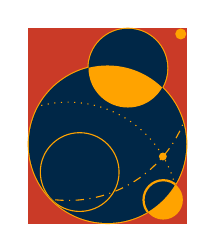
\begin{tikzpicture}
        \def\rOne{1}
        \def\rTwo{0.5}
        \def\rThree{0.25}
        \def\angleOne{75}
        \def\angleTwo{-45}
        
        \def\maincolor{uninablue}
        \def\linecolor{cheddar}
        \def\backgroundcolor{myorange}

        % fill background
        \fill [\backgroundcolor] 
            (-\rOne-0.013, -\rOne-0.012) rectangle 
            (\rOne+0.013, \rOne + 0.48)
        ;

        \draw [thick, \linecolor] (0, 0) circle (\rOne);
        \draw [thick, \linecolor] (\angleOne:\rOne) circle (\rTwo);
        \fill [\linecolor] (\angleTwo:\rOne) circle (\rThree);
        \fill [\linecolor] (\rOne - 0.07, \rOne + 0.4) circle (0.07);
        
        \fill [\maincolor] (0, 0) circle (\rOne);
        \fill [\maincolor] (\angleOne:\rOne) circle (\rTwo);
        \clip (0, 0) circle (\rOne);
        \fill [\linecolor] (\angleOne:\rOne) circle (\rTwo);
        
        \draw [thick, \linecolor] (\angleTwo:\rOne) circle (\rThree);
        \draw [dashdotted, \linecolor] (120:\rOne) circle (1.58);
        \draw [dotted, \linecolor] (-120:\rOne) circle (1.4);
        \fill [\linecolor] (-12.5:0.72*\rOne) circle (0.05);
        \draw [\linecolor] (45:-0.5) circle (0.5);
    \end{tikzpicture}
\end{document}